% /Users/pikachu/books/payments-book/src/parts/part4/ch19-fraud.tex
\chapter{Фрод: кто атакует и как защищаться}
\label{ch:fraud}
\margintoc

\begin{kaobox}[title=Что вы узнаете из этой главы]
  Антифрод не сводится к одному алгоритму. Это система слоёв, где
  каждый следующий слой закрывает то, что пропустил предыдущий.
  В этой главе мы разберём основные виды мошенничества с платёжными
  картами, их типовые уязвимости, пороговые проверки частоты
  (velocity checks), цифровой слепок устройства (device
  fingerprinting), модель машинного обучения (machine learning,
  ML), гибридный скоринг и цену ложноположительного срабатывания
  (false positive).
\end{kaobox}

Главный вопрос этой главы звучит просто: как отличить легитимную
транзакцию от атаки, если атакующий уже научился копировать внешний
вид нормального поведения? Пример знаком каждому, кто работает с
платежами: клиент хочет оплатить покупку, злоумышленник ищет слабое
место, а риск-команда должна не только поймать атаку, но и не
переборщить с блокировками. Механизм защиты здесь всегда один и тот
же по форме, хотя меняется по содержанию: мы смотрим на следы
устройства, историю аккаунта, частоту попыток и поведение после
платежа. Ограничение тоже очевидно: чем строже фильтр, тем выше цена
ошибочного отказа. Вывод отсюда простой: антифрод -- это не запрет
на всё подозрительное, а поиск разумного баланса.

\section{Карта угроз}
\label{sec:fraud-threats}

Мошенничество с платёжными картами -- это индустрия со
своими рынками, ролями и специализацией. Примером служит любая
теневая площадка, где данные карт продаются, проверяются и снова
упаковываются в атаку. Механизм понятен: разные злоумышленники
эксплуатируют разные слабые места, а значит и контрмеры должны
быть разными. Ограничение у защиты простое: если смотреть только на
один тип сигнала, часть атак неизбежно пройдёт мимо. Вывод: сначала
надо понять природу атаки, а уже потом строить фильтр.

Самый старый класс атак -- скимминг. Пример прост: накладка на
POS-терминале или банкомате считывает данные магнитной полосы и
передаёт их злоумышленнику. Механизм тоже прозрачен: украденные
данные, или дампы (dumps), продают на закрытых площадках, после чего
из них делают клон карты и пытаются провести операции там, где ещё
разрешён откат на магнитную полосу. Ограничение у этой схемы есть,
и оно важное: EMV-чип резко снижает ценность такого клона, потому что
криптограмма формируется заново для каждой транзакции и не
воспроизводится. Вывод: пока живёт fallback на магнитную полосу,
скимминг нельзя считать побеждённым окончательно \sidecite{emvco-book1}.

Следующий по масштабу класс атак -- мошенничество без предъявления
карты (card-not-present, CNP) и карточный перебор (carding). Пример
здесь знаком по e-commerce: у атакующего есть PAN, срок действия и CVV,
полученные из утечки, через фишинг, из вредоносного ПО или на теневом
рынке. Механизм атаки строится на мелких проверочных транзакциях:
если данные проходят на символических суммах, после этого делается
крупная покупка. Ограничение у злоумышленника то же, что и у защиты:
чем больше попыток и чем плотнее след, тем заметнее аномалия. Вывод:
пороговые проверки частоты как раз и нужны, чтобы ловить такие пробы
до того, как они превратятся в серьёзный ущерб.

Отдельный класс атак -- захват учётной записи (Account Takeover, ATO).
Пример понятен: злоумышленник входит в уже существующий аккаунт
клиента. Механизм обычно один из трёх: подстановка утёкших пар
логин/пароль (credential stuffing), фишинг или социальная инженерия;
иногда добавляется подмена SIM-карты. После этого атакующий получает
доступ к сохранённым картам, адресам доставки и истории покупок.
Ограничение для защиты в том, что такая транзакция выглядит почти
легитимной: тот же аккаунт, та же карта, нередко то же устройство.
Вывод отсюда такой: любые резкие смены устройства, географии или
адреса доставки должны включать дополнительную проверку.

Совершенно иная природа у дружественного фрода (friendly fraud).
Пример здесь банален и поэтому опасен: держатель карты сам делает
покупку, получает товар или услугу, а потом спорит транзакцию и
заявляет, что это был не он. Механизм не требует взлома; достаточно
злоупотребить процедурой chargeback. Чаще всего это происходит с
цифровыми товарами: играми, подписками, программным обеспечением,
потому что доказать факт использования там труднее. Ограничение для
защиты тоже очевидно: если у мерчанта нет следов предыдущего
поведения, спор превращается в слово против слова. Вывод: именно
поэтому полезны программы доказательства участия клиента в
предыдущих операциях, о которых мы говорим в главе \ref{ch:disputes}.

Наконец, наиболее коварный вид -- bust-out-мошенничество. Пример
всегда один и тот же: злоумышленник сначала выглядит добросовестным
клиентом или мерчантом, накапливает хорошую историю, а потом резко
увеличивает объём операций, выбирает деньги и исчезает. Механизм в
эмитентском контуре похож на классический кредитный обман: несколько
карт, аккуратное поведение, рост лимитов и затем дефолт. В эквайринге
схема выглядит иначе, но логика та же: подключение мерчанта, спокойный
старт, резкий рост оборота, отказ от возвратов и уход. Ограничение
защиты здесь состоит в том, что короткое наблюдение почти ничего не
показывает. Вывод: такие случаи можно ловить только через полноценную
проверку мерчанта и последующий поведенческий мониторинг.

Эта карта угроз нужна не ради таксономии. Её практический смысл
состоит в том, что каждой атаке соответствует свой объект наблюдения:
где-то нужно смотреть на устройство, где-то на аккаунт, где-то на
историю владения товаром, а где-то на аномалию мерчанта. Антифрод
начинает работать только тогда, когда контрмера соотнесена с
конкретной уязвимостью. Абстрактного подозрения для настройки недостаточно.

\section{Первая линия: пороговые проверки и статические правила}
\label{sec:fraud-rules}

Какая защита срабатывает первой? Обычно это пороговые проверки
(velocity checks) и статические правила. Пример у них всегда один и
тот же: слишком много операций с одного IP, слишком много попыток с
одной карты, слишком много разных карт на одном устройстве или
неестественный скачок суммы по сравнению с историей клиента.
Механизм прост до предела: правило сравнивает текущую операцию с
заданным порогом и мгновенно решает, пропускать её дальше или нет.
Ограничение также известно заранее: если пороги задать слишком
жёстко, правила начнут резать обычных клиентов; если слишком мягко,
они перестанут ловить атаку. Вывод: правила нужны как дешёвая первая
линия отсечения. Заменой остальному антифроду они не становятся.

Типичные правила выглядят так: более N транзакций с одного IP за
час, более M транзакций с одной карты за десять минут, более K
попыток с одного устройства за сутки или сумма, которая резко
выбивается из истории аккаунта. Каждое такое правило дёшево,
быстро и удобно для интерпретации. Его легко объяснить комплаенсу,
показать регулятору и отладить в оперативном хранилище.

Преимущества здесь очевидны: предсказуемость, объяснимость и
минимальная задержка. Ограничения тоже не скрыты: атакующие быстро
научаются дробить поток под пороги, а правила не понимают контекст.
Крупная покупка в аэропорту перед вылетом для одного клиента
нормальна, а для другого будет сигналом риска. Вывод: статические
правила хороши как грубый фильтр, но плохи как единственный судья.

Особая категория здесь -- проверки карточного перебора (carding
checks). Пример знаком всем, кто видел живой fraud-стрим: серия
мелких тестовых списаний с одного IP или устройства, иногда по
разным картам, за короткий промежуток времени. Механизм у атаки
такой: сначала проверить, какие данные ещё живы, а потом перейти к
крупной операции. Ограничение для атакующего в том, что такой
рисунок трудно скрыть полностью. Вывод: именно по этой причине
проверки тестовых сумм остаются одними из самых эффективных в
пороговом слое.

\section{Цифровой слепок устройства и поведенческая аналитика}
\label{sec:fraud-fingerprint}

Что даёт цифровой слепок устройства (device fingerprinting)? Он
собирает набор признаков браузера или телефона и по их комбинации
позволяет распознать именно устройство. Человека как такового этот метод не идентифицирует.
Примером служат User-Agent, размер экрана, набор шрифтов, часовой
пояс, возможности WebGL, canvas- и audio-отпечатки. Механизм здесь
вероятностный: по одному признаку устройство не узнать, но по набору
можно получить почти уникальную комбинацию. Ограничение очевидно:
если браузер специально скрывает или рандомизирует признаки, точность
падает. Вывод: fingerprinting полезен не как абсолютный идентификатор,
а как ещё один устойчивый сигнал риска.

Ценность такого слепка -- в привязке устройства к истории операций.
Если один и тот же слепок месяцами участвует в нормальных покупках,
это укрепляет доверие. Если новый слепок сразу пытается провести
дорогую операцию на новом адресе доставки, это уже сигнал риска.
Именно такая логика лежит в основе программ доказательства участия
клиента в предыдущих операциях.

Поведенческая аналитика добавляет сюда данные текущей сессии:
скорость набора, траекторию мыши, время заполнения формы и паузы
между действиями. Пример здесь бытовой, но показательный: человек,
который вводит чужую карту по памяти, часто замедляется и ошибается,
а скриптовый бот, наоборот, оставляет слишком ровный след. Механизм
работает пассивно и не добавляет лишнего трения в оформление покупки.
Ограничение, однако, тоже есть: если клиент пользуется
privacy-браузером или если атакующий умеет имитировать движение,
сигнал слабеет. Вывод: поведенческие признаки лучше всего работают
вместе со слепком устройства и плохо заменяют его полностью.

На мобильных платформах для сопоставимого уровня данных нужен
отдельный SDK, а часть браузеров и расширений специально искажает
атрибуты. Тем не менее для обычного фродового потока слепок
устройства остаётся полезным: его трудно подделать полностью, но
ещё труднее сделать это незаметно.

\section{Машинное обучение в антифроде: что работает, а что переоценено}
\label{sec:fraud-ml}

Когда правил уже мало, в дело вступает машинное обучение. Пример
здесь тот же самый: карта до атаки вела себя нормально и не попала
под пороговые проверки, но в сумме признаков -- время суток, сумма,
география, расстояние от предыдущей операции -- возникает редкая
комбинация. Механизм модели состоит в том, чтобы искать не один
подозрительный признак, а целый паттерн. Ограничение тоже знакомо:
модель видит только то, чему её научили, и плохо переживает смену
поведения злоумышленников. Вывод: ML полезен там, где правила уже
слишком грубы, но ему нужен постоянный контроль качества.

На практике важнее качество признаков, чем модная архитектура.
Чаще всего хорошо работает градиентный бустинг: он проще в обучении,
лучше объясняется и обычно достаточно силён для производственного
антифрода. Признаки при этом остаются вполне земными: окна по
времени, агрегаты по мерчанту, скользящие суммы, расстояние от
предыдущей транзакции. Это совпадает и с открытой литературой:
для табличных fraud-датасетов сильными базовыми моделями остаются
деревья и градиентный бустинг, а качество признаков и их отбор
заметно влияют на итоговые precision/recall не меньше, чем выбор
конкретной архитектуры \sidecite{fraud-feature-selection-2024}\sidecite{fraud-lightgbm-2024}.

Ключевая операционная проблема здесь -- дрейф концепции (concept
drift). Мошенники подстраиваются под то, что модель уже научилась
ловить, и через несколько недель вчерашний сигнал перестаёт
работать. Модель, которая давно не переобучалась, начинает
деградировать. Хороший антифрод-пайплайн поэтому устроен как
процесс. Разовая установка здесь не работает: контроль качества по
скользящему окну, регулярное переобучение и проверка новых версий
на отложенных данных.

Ещё одна ловушка -- дисбаланс классов. В реальном потоке
легитимных операций почти всегда гораздо больше, чем мошеннических,
поэтому простая точность ничего не говорит о качестве. Модель,
которая всегда отвечает «легитимно», формально выглядит почти
идеальной, но фактически бесполезна. Поэтому в антифроде смотрят
на precision, recall и их компромисс через F1 или PR-AUC. Вывод
здесь простой: accuracy удобна для отчёта, но почти бесполезна
для защиты.

Отдельное требование -- объяснимость. Клиенту и клиентскому сервису
нужна понятная причина отказа. Ответ в духе «модель сказала нет» здесь не годится. Поэтому
в производстве используют объясняющие методы вроде SHAP и LIME,
которые показывают вклад отдельных признаков в итоговое решение.

\section{Гибридные системы: правила и модель}
\label{sec:fraud-hybrid}

Почему почти всегда нужна гибридная схема? Потому что ни правила,
ни модель по отдельности не дают полного ответа. Правила хорошо
ловят очевидные атаки, но плохо видят сложные комбинации признаков.
Модель видит больше, но требует обучения, наблюдения и объяснения.
Вывод отсюда давно известен промышленным командам: сначала грубый
отсев, потом скоринг, потом отдельные правила на итоговый результат.

Стандартный промышленный поток выглядит так. Сначала идёт
предварительный отсев (pre-screening): быстрые правила блокируют
совсем очевидные случаи, например карточный перебор, карту из
стоп-листа или явное превышение порога частоты. Затем работает
скоринговый модуль (scoring engine): модель выдаёт оценку риска
для того, что прошло первичный фильтр. После этого вступают
правила после скоринга (post-scoring rules): высокие значения
ведут к блокировке, средние могут потребовать дополнительную
верификацию или 3DS-проверку, низкие проходят дальше. Механизм
здесь важнее словаря: каждый слой отвечает за свой тип решения.

\begin{marginfigure}
  \centering
  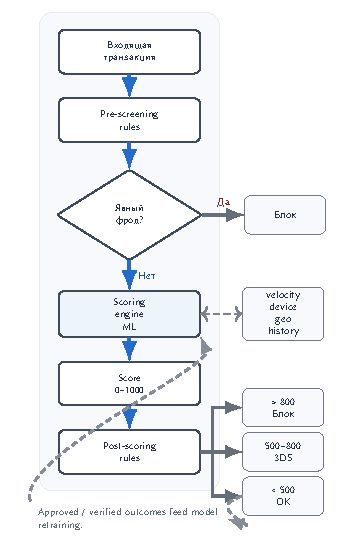
\includegraphics[width=\linewidth]{assets/figures/ch19-fraud/fraud-hybrid.pdf}
  \caption{Гибридная система антифрода: правила и скоринг.}
  \label{fig:fraud-hybrid}
\end{marginfigure}

Обратная связь в такой схеме критична. Исходы транзакций, ручные
верификации и спорные случаи должны возвращаться в обучающую
выборку. Без этого модель постепенно слепнет: вчерашние атаки она
видит, а сегодняшние -- уже нет.

\section{Скоринг и 3DS RBA}
\label{sec:fraud-3ds-rba}

В главе \ref{ch:3ds} мы уже видели риск-ориентированную аутентификацию
(Risk-Based Authentication, RBA) как способ принятия решения в 3DS v2:
ACS эмитента решает, требовать дополнительную проверку или
разрешить авторизацию без дополнительного подтверждения.
Для мерчанта возникает естественный вопрос: как передать эмитенту
контекст, который улучшит его решение?

В 3DS v2 запрос аутентификации содержит поле \enquote{requestor risk
indicator} -- структурированный набор атрибутов, который мерчант
передаёт в ACS: сумма, тип транзакции, имя аккаунта, история
предыдущих операций, устройство, доставка. ACS использует эти данные
вместе с собственной моделью эмитента \sidecite{emvco-3ds}.

Связка выглядит так: антифрод мерчанта вычисляет score; при высоком
score мерчант передаёт в 3DS-запрос сигнал о высоком риске и просит
дополнительную проверку; ACS получает этот контекст и, если его
собственная оценка не противоречит, тоже требует дополнительную
проверку. При низком score мерчант, напротив, сигнализирует о
легитимной операции и просит авторизацию без дополнительного
подтверждения; эмитент может согласиться, если его собственная
модель не видит проблемы. Это кооперативный протокол: ни мерчант, ни
эмитент не
контролируют исход в одностороннем порядке, но входные данные
мерчанта влияют на результат.

На стороне схем работают собственные сервисы риск-оценки: они
собирают дополнительный сигнал по транзакции и помогают эмитенту
не путать легитимный поток с серией тестовых и атакующих попыток.
Для мерчанта это ещё один входной сигнал в авторизационной логике,
а не прозрачная магия \sidecite{visa-core-rules}\sidecite{mc-rules}.

\section{Ложноположительное срабатывание как скрытая потеря}
\label{sec:fraud-false-positive}

Что дороже: пропустить мошенничество или ошибочно заблокировать
легитимного клиента? Ответ неприятен именно своей двойственностью:
антифрод, который не пропускает ни одной атаки, обычно блокирует
и слишком много нормальных операций. Идеал ясен, но недостижим:
нужна система, которая удерживает баланс между ложноположительным
срабатыванием (false positive) и ложноотрицательным срабатыванием
(false negative).

Большинство команд интуитивно смотрят только на пропущенный фрод.
Это понятно: каждая мошенническая операция -- прямой убыток, часто
переходящий в chargeback. Но у ошибки первого рода есть собственная
цена, и она нередко скрыта в операционных расходах.

Когда легитимная транзакция ошибочно блокируется, клиент вынужден
обращаться в поддержку, а мерчант теряет не только текущую оплату,
но иногда и будущие покупки. Именно поэтому ложноположительные
срабатывания нужно считать в деньгах, а не ограничиваться процентами отчёта.

ROC- и PR-кривые помогают увидеть этот компромисс на графике.
Двигаясь по ним, команда меняет порог решения: ниже порог -- больше
блокировок и меньше мошенничества, но выше число ошибочных отказов;
выше порог -- наоборот. Оптимальная точка зависит от экономики
продукта. Для цифровых товаров, где себестоимость доставки мала,
можно позволить себе более строгий фильтр. Для физической доставки
и дорогого возврата порог обычно приходится смягчать.

\begin{kaobox}[title=На практике]
  Считайте стоимость false positive явно. Для каждого заблокированного
  легитимного клиента -- это (1) упущенная транзакция; (2) вероятность
  потери клиента навсегда (умножить на LTV); (3) операционные затраты
  на поддержку. Сравните эту сумму с ожидаемыми потерями от фрода при
  снижении порога. Часто именно такой расчёт показывает, что система
  настроена заметно агрессивнее, чем нужно бизнесу.
\end{kaobox}

\begin{chaptersummary}
\begin{itemize}
  \item Пять основных видов атак -- скимминг, CNP/carding, ATO,
        дружелюбный фрод и bust-out -- эксплуатируют разные уязвимости
        и требуют разных контрмер.
  \item Пороговые проверки и статические правила -- самый дешёвый слой
        антифрода; они ловят очевидные аномалии, но плохо понимают контекст.
  \item Машинное обучение работает там, где один признак мало что
        решает; дрейф концепции и дисбаланс классов требуют постоянного
        контроля качества.
  \item Гибридная архитектура обязательна: сначала быстрый отсев,
        затем скоринг, затем отдельные правила на итоговый результат.
  \item Скоринг антифрода и риск-ориентированная аутентификация в 3DS
        работают как кооперативный протокол между мерчантом и эмитентом.
  \item Ложноположительное срабатывание нужно считать в деньгах,
        а не только в процентах ошибок.
\end{itemize}
\end{chaptersummary}
